92. \begin{figure}[ht!]
\center{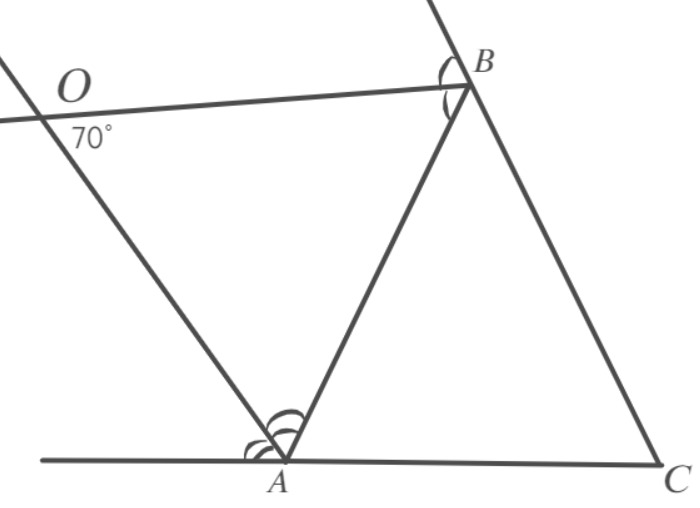
\includegraphics[scale=0.35]{g92.png}}
\end{figure}\\
Обозначим $\angle A=\angle C=x,$ тогда $\angle B=180^\circ-2x.$ Запишем сумму углов треугольника $AOB:\ 70^\circ+(180^\circ-x):2+(180^\circ-(180^\circ-2x)):2=180^\circ,\ 70^\circ +90^\circ-\frac{1}{2}x+x=180^\circ,\ \frac{1}{2}x=20^\circ,\ x=40^\circ.$ Значит углы треугольника $ABC$ равны $40^\circ,\ 40^\circ$ и $180^\circ-2\cdot40^\circ=100^\circ.$
ewpage
oindent
